Задача хорошо сводится к оптимизационной задаче с большим количеством параметров.
Причём на обработку одного изображения можно выделить много времени и вычислительных ресурсов — главное — результат.

Таким образом, решено было использовать эвристические алгоритмы оптимизации:
«Генетический алгоритм» (ГА) и «Симуляция отжига».
ГА хорошо справляется с избеганием совсем локальных оптимумов и нахождением более хороших решений,
а отжиг может улучшить приближение, полученное с помощью ГА за счёт более высокой скорости сходимости
(используется отжиг, а не, например, градиентный спуск, так как считать градиент в данном случае затруднительно
(но его поддержка планируется, см.~\ref{subsec:local-methods})).
(Исследования, которые я читал, показывают, что для большого количества стандартных задач комбинаторной оптимизации
ГА показывает лучшие результаты среди алгоритмов оптимизации (ссылка есть в секции~\ref{sec:opimization_algorithms}))
Подробное описание алгоритмов, моей их реализации, и улучшений представлено в секции~\ref{sec:opimization_algorithms}.


\subsection{Представление «решения»  — набора мазков}
Программа работает с последовательностями мазков, находя лучшую из них.
Однако, чтобы алгоритм оптимизации работал с ними, наборы мазков должны быть представлены в виде векторов в $\mathbb{R}^n$.

Каждый мазок является кривой Безье второго порядка:

\begin{equation}\label{eq:bezier_curve}
    \begin{cases}
        x(t) = {p_1}_x + (1 - t)^2 \cdot (p_0 - p_1)_x + t^2 \cdot (p_2 - p_1)_x \\
        y(t) = {p_1}_y + (1 - t)^2 \cdot (p_0 - p_1)_y + t^2 \cdot (p_2 - p_1)_y
    \end{cases}
\end{equation}

И задаётся с помощью семи параметров — вещественных чисел.
Формат данных в «геноме» таков:

\begin{figure}[h!]
    \centering
    \adjincludegraphics[width=0.7\textwidth, clip, trim={0.15\width} {0.7\height} {0.15\width} {0.125\height}]{genome_contents_table.pdf}
    \caption{Схема хранения генома}
    \label{fig:genome_contents_table}
\end{figure}
\FloatBarrier


, где $p_{n_x} ~\&\&~ p_{n_y}, n \in \{ 0, 1, 2 \}$ — координаты направляющей точки под номером n (из всего 3 у каждого мазка),
а \textit{width}  — толщина мазка.

Здесь нет параметра  «цвет».
Причина объяснена в разделе:~\ref{subsec:color_in_genome}.

\subsection{Задание функции ошибки}
Чтобы решить задачу алгоритмом оптимизации, нужна некая метрика — функция, которая будет определять степень «неподходящести» данного ей решения.
Именно она будет передаваться алгоритму оптимизации.
В нашем случае вычисление функции ошибки (далее — ФО) включает в себя растеризацию мазков (отображение их на изображении) и вычисления, производящие сравнения полученного результата с желаемым.
ФО необходимо задать таким образом, чтобы она отражала качество полученной комбинации мазков,
причём в любой точке направление её уменьшения соответствовало направлению улучшения результата.
За основу была выбрана \href{https://en.wikipedia.org/wiki/Mean_squared_error}{MSE} (Mean Square Error):

\begin{equation}\label{eq:equation}
    MSE = \frac{1}{width \cdot height} \cdot \sum_{y = 0}^{y < height} { \sum_{x = 0}^{x < width} { \sum_{c \in  \left\{ r, g, b \right\} } { \left( {\overrightarrow {rendered_{x, y}}}_c - {\overrightarrow{original_{x, y}}}_c\right)^2 }}}
\end{equation}

MSE — универасльная мертрика для схожести изображений, она повсеместно используется при работе с ними.
Но в нашем случае, о чём свидетельствует практика, целесообразно добавить в ФО компоненту, «наказывающую» за наложение мазков друг на друга, а также за пустые (ничем не закрашенные) места.

Первое улучшение очевидно — при прочих равных лучше ситуация, при которой та же картина достигнута с меньшим использованием краски
(а если не вводить эту компоненту, наложено в найденном решении может быть сразу много (> 2) мазков в одной точке).
Если нет разницы, зачем переплачивать?

С теоретической точки зрения может быть непонятна надбавка за пустоты: ведь если место пустое, оно и так не даёт оптимальное MSE.
Однако на практике пусто́ты недостаточно быстро и полно покрываются (особенно — на ускоренном режиме) без этой надбавки.

Таким образом, функция ошибки сделана так, чтобы максимально стимулировать правильно распределение мазков.

\subsection{Растеризация мазков}\label{subsec:rasterization}
Имея мазок, заданный в виде трёх точек на плоскости, толщины и цвета, нужно уметь его отобразить его на «холсте», то есть в виде набора пикселей.
Это нужно, чтобы подсчитать функцию ошибки для заданного набора мазков,
причём так, чтобы результат максимально соответствовал мазку, рисуемому роботом.
В качестве достаточно точной модели описания такого мазка возьмём круглую кисть, перемещающуюся по заданной траектории.
Есть много способов произвести растеризацию.
Нужно выбрать тот, который будет производительным и в то же время максимально близким к реальному мазку.

Самый простой — для некоторого количества точек на кривой Безье (с достаточно маленьким шагом, примерно один пиксель) проводим вертикальную линию: вверх на width и  вниз — тоже.
Это даёт высокую производительность и сносно выглядит на участках, близких к горизонтальным, но результат, полученный таким способом, очень далёк от реальности на вертикальных участках:
\begin{figure}[h!]
    \centering
    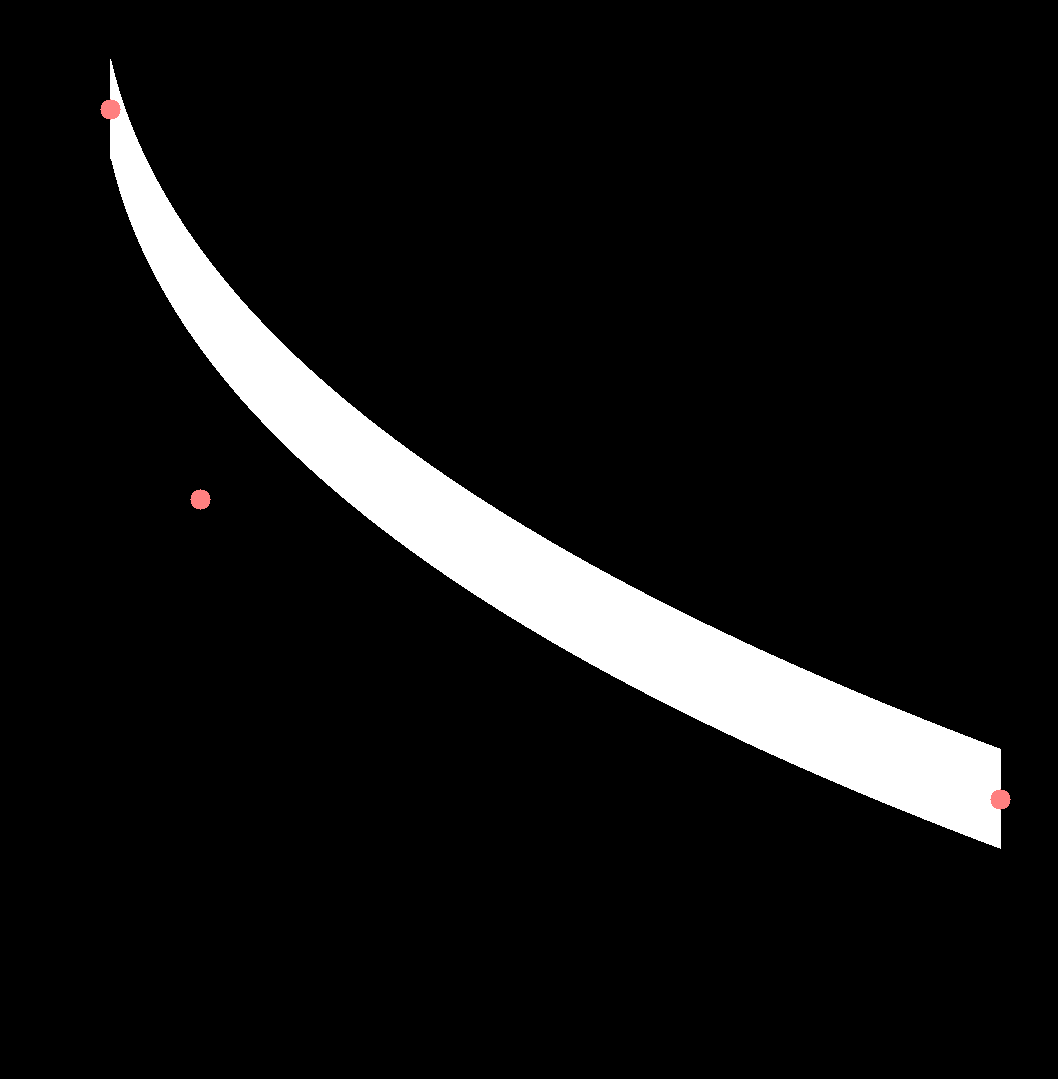
\includegraphics[width=0.75\textwidth]{stroke_vertical.png}
    \caption{(Красным обозначены точки, задающие кривую)}
    \label{fig:vertical_stroke}
\end{figure}
\FloatBarrier


\begin{figure}[h!]
    \centering
    
\includegraphics[width=0.75\textwidth]{one_stroke.png}
    \caption{Иногда такой способ добавляет свой шарм}
    \label{fig:pretty_vert_stroke}
\end{figure}
\FloatBarrier


Есть разные способы избавиться от этих недостатков, сохраняя максимальную производительность.
Например:
\begin{itemize}
    \item Совмещать горизонтальные и вертикальные полосы
    \item Проводить полосы перпендикулярно направлению кривой в данной точке
\end{itemize}
В каждом из них будут наблюдаться пустые места, полости, что недопустимо.

Ультимативным же способом является подражание реальной жизни: «проведение» круглой «кистью» по экрану.
То есть берутся точки на кривой на небольшом расстоянии друг от друга, далее из каждой рисуется круг радиусом width.
Однако в таком случае каждая точка, попадающая в мазок, обрабатывается много раз (для близких кругов), что значительно замедляет рендерниг.
Если же увеличить шаг, этой проблемы можно частично избежать, но мазок стал бы неровным.
При маленьком шаге это выглядит так:
\begin{figure}[h!]
    \centering
    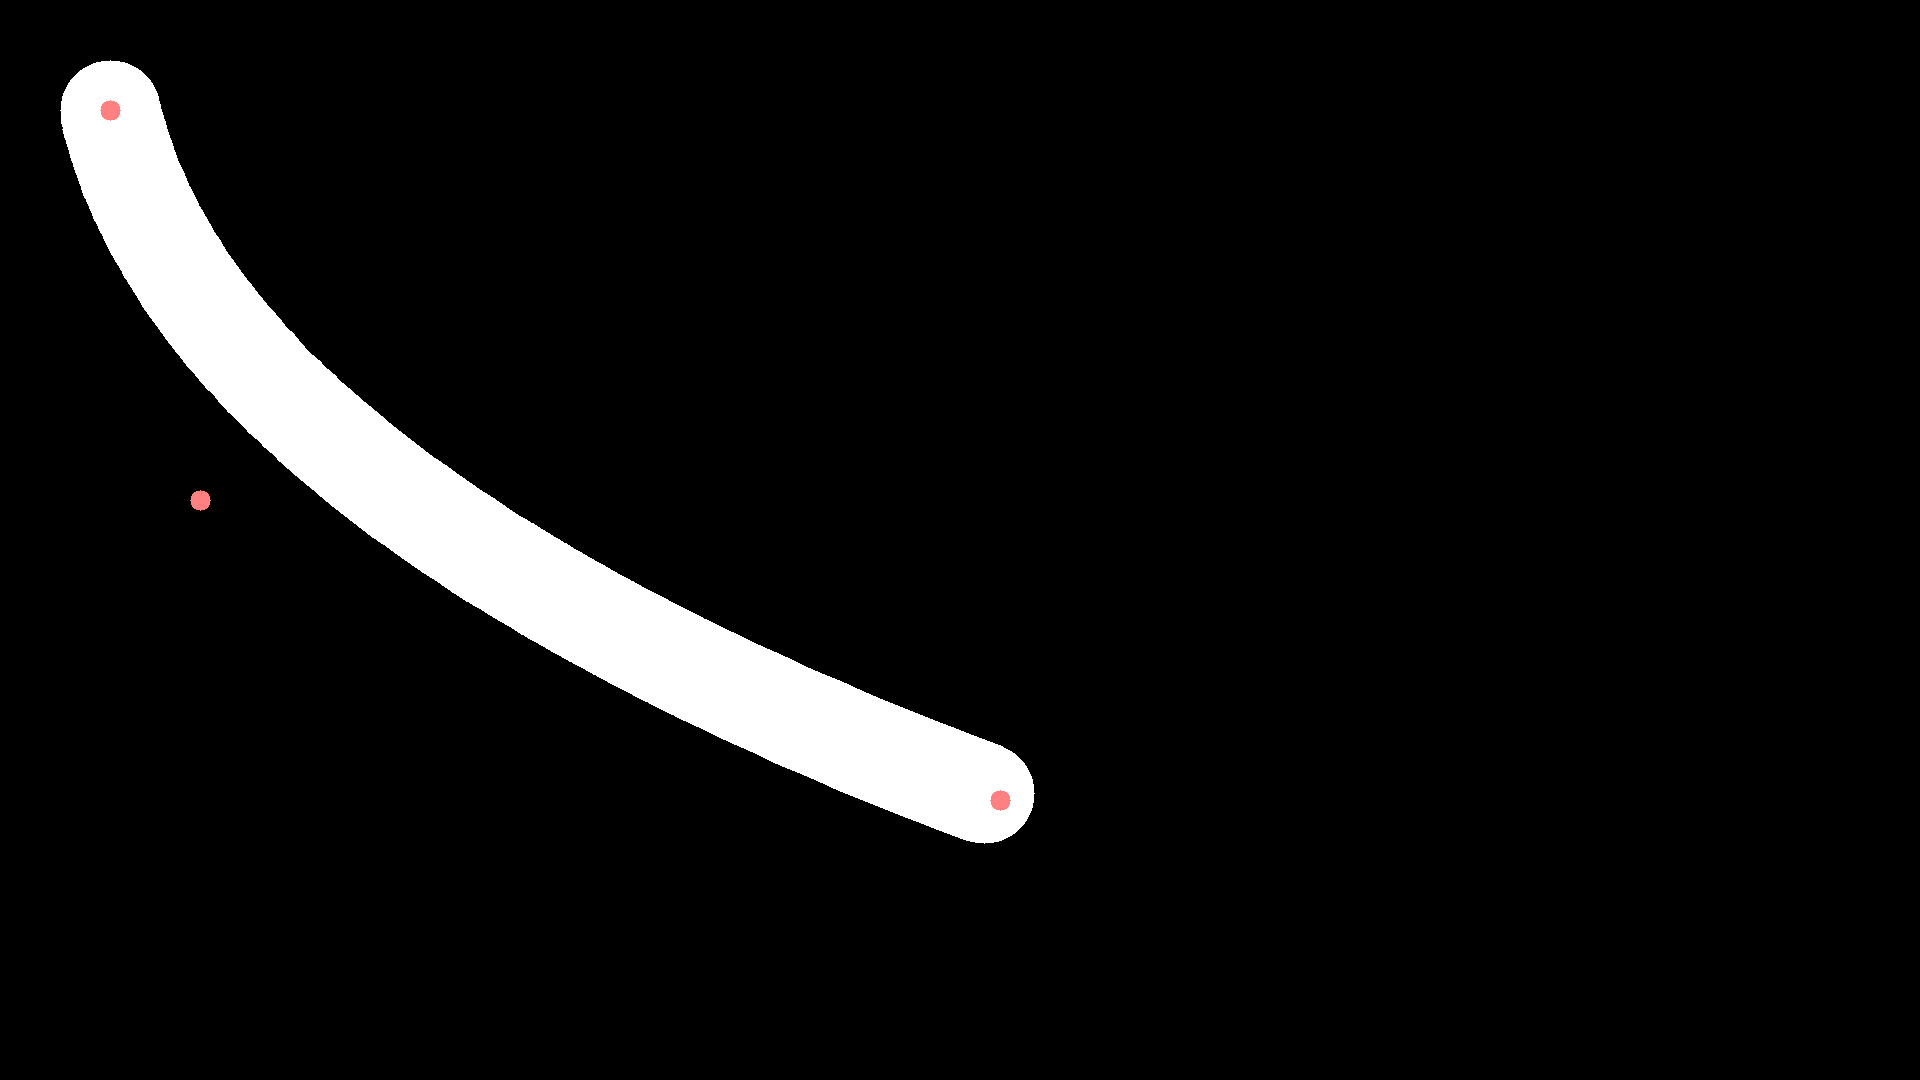
\includegraphics[width=0.75\textwidth]{stroke_smooth.png}
    \label{fig:smooth_stroke}
\end{figure}
\FloatBarrier

В будущем планируется улучшить алгоритм для ускорения растеризации при почти том же качестве.
Рассматриваются варианты:
\begin{itemize}
    \item Заменить круглую кисть на также гладкую, но с более медленным закруглением с дальней от вектора кривой в данной точке стороны, поворачивая кисть соответствующим образом:
    \begin{figure}[h!]
        \centering
        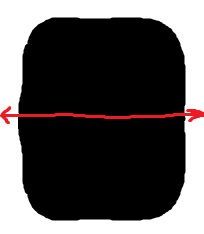
\includegraphics[width=0.75\textwidth]{modern_brush.png}
        \caption{(красным обозначено направление вектора кривой)}
        \label{fig:modern_brush}
    \end{figure}
    \FloatBarrier

    Такое изменение поможет уменьшить артефакты при увеличении шага между точками на кривой, то есть позволит сделать шаг больше, ускорив процесс.

    \item Автоматически разбивать мазок на «полигоны».
                Для этого нужно пройтись по кривой и с некоторым шагом (уже побольше, чем раньше),
                отметить для каждой рассматриваемой точки на прямой, содержащей её и перпендикулярной текущему направлению, точки в обе стороны от неё на расстоянии width.
                Каждая из них добавляется в соответствующий стороне в порядке обхода список.
                Потом полигоны, полученные из соседних точек на кривой и соответствующим им вынесенным точкам, заливаются нужным цветом.
                На концах же мазка рендерятся круги.

    \begin{figure}[h!]
        \centering
        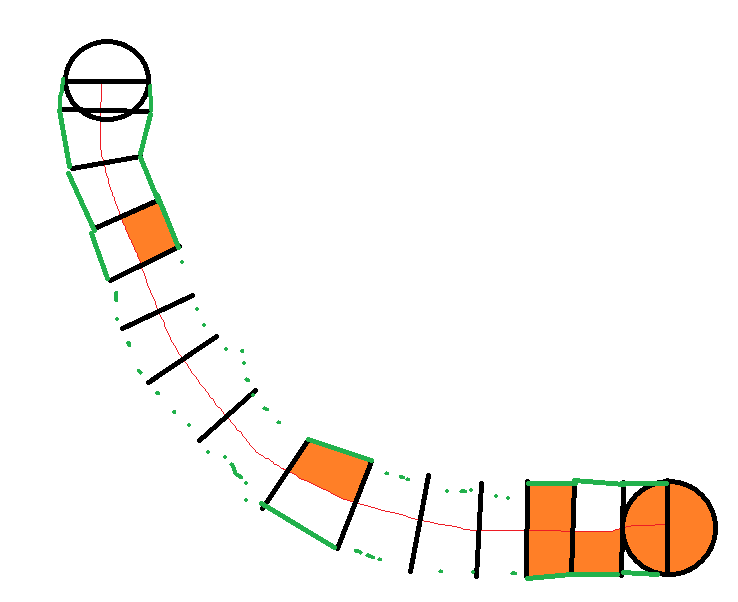
\includegraphics[width=0.75\textwidth]{polygonal_stroke.png}
        \caption{Схема полигональной разбивки мазка}
        \label{fig:polygonal_stroke}
    \end{figure}
    \FloatBarrier

    При использовании этого метода никакая существенная часть пикселей мазка не обрабатывается много раз, что говорит о высокой эффективности алгоритма.
    Поэтому я собираюсь внедрить такой метод в ближайшее время.
\end{itemize}

Что же касается совместимости с видеокартой,
для круга и модифицированной кисти легко определить bouding-box,
и несложно по координатам пикселя быстро определить, принадлежит ли он этому примитиву.
А рендеринг полигонов производится аппаратно.

Подробнее про внедрение видеокарты можно почитать в разделе \ref{subsec:move_graphics_to_videocard}.

\subsection{Проведение операций ГА}\label{subsec:ga-operations}

Задачу можно представить чисто математически — как оптимизации функции $\mathbb{R}^n \longleftarrow \mathbb{R}$.
Несмотря на то, что в пределе такой подход приведёт к некоторому результату,
\begin{itemize}
    \item Это займёт очень много времени
    \item Результат не будет соответствовать некоторым критериям из реальной жизни
\end{itemize}

Операции, по умолчанию производящиеся в ГА, несколько изменены и адаптированы для конкретной задачи.



Важная проблема решения «в лоб» (которую нужно устранить именно так) — то, что, если разрешить в качестве области поиска
по каждой координате указать весь диапазон изображения по этой координате, типичный мазок будет растянут на всю картину.
Но, во-первых, настоящие мазки — совсем не такие — они существенно меньше изображения.
Во-вторых, понятно, что алгоритму будет несравнимо более сложно найти нужную комбинацию мазков.
Например, потому, что она, скорее всего, будет предполагать малый размер мазков, который, конечно,
возможен при такой постановке задачи, однако алгоритму потребуется огромное количество ресурсов, чтобы достичь его.

Поэтому рассмотрение координат разных точек как совершенно независимых параметров — плохая идея.
Я решил составить набор ограничений на разные параметры мазков:
\begin{itemize}
    \item Минимальные и максимальные высота и ширина bounding\_box-а мазка
    \item Минимальные и максимальные толщина и длина мазка
    \item Всписываемость в изображение
    \item Искривлённость
\end{itemize}

Для каждого параметра необходимо уметь:
\begin{itemize}
    \item Определять, правда ли, что заданный мазок подходит по ограничения
    \item «Подправлять» мазок так, чтобы значения параметров пришли в норму
    \item Случайно генерировать набор мазков, чтобы все соответствовали критериям
\end{itemize}
Насчёт второго пункта важно отметить: мутации точек по амплитуде — в среднем заметно меньше размера самих мазков,
поэтому от методов корректировки не нужно очень высокое качество (например, какие-то гарантии сохранения формы или центра или чего-то ещё):
неидеальности корректировки — тоже часть мутаций — небольших случайных изменений.

В случае с координатами — рассматривается bounding-box мазка.
Когда происходит корректировка по каждой из координат, если bounding-box не помещается в изображение по этой координате,
мазок перемещается по ней так, что точки на «дельней» границе «отражаются» от соответствущей границы изображения, но
со случайным «коэффициентом отражения» $k \in [0; 0.5]$.

А именно — новое место для них находится на перпендикуляре к краю изображению,
проходящем через изначальное положение этих точек, и удалено от границы на $k \cdot d_0$, где $d_0$ — расстояние от границы до изначальной точки.
Иначе говоря, $new\_coord = image\_border_{coord} + k \times (image\_border_{coord} - old\_coord)$
То есть чем дальше мазок вышел за границу, чем дальше его «отбросит».
Однако типичная мутация мала по сравнению с размерами изображения, поэтому не стоит ожидать, что выбившиеся мазки вдруг выползут на центр (и это хорошо).
% Всё это можно было бы назвать гомотетией с коэффициентом -k, если бы форма мазка была перевёрнутой, и он уменьшался.

Случайный и ненулевой вес нужен, чтобы не наблюдалось скопление мазков по краям.

Затем (для подстраховки) по каждой координате каждой точки просто делается обрезка по диапазону \{ 0, max_coord \}.

В случае с размерами bounding\_box-а точки, если что-то не так для какой-то из координат, происходит scaling точек мазка по этой координате так,
чтобы он соответствовал ближайшему разрешённому значению
(то есть если размер слишком большой — верхней границе (max_{d_{coord}}), если слишком малый — нижней (min_{d_{coord}})).

Тощина просто обрезается по разрешённым границам.

Длина просто считается, и, если вдруг она слишком велика или мала
(хотя это маловероятно, если подходит под bounding box, а если и так и происходит, то превышение или преуменьшение всё равно незначительное)
Длина кривой определяется классическим образом, по этой формуле:
\begin{equation}\label{eq:curve_length}
    L = \int \limits_{a}^{b}{ \sqrt {{x'}^{2}(t) + {y'}^{2}(t)} } dt
\end{equation}

Применение этого к кривым безье можно найти здесь: \url{https://members.loria.fr/samuel.hornus/quadratic-arc-length.html}

Про регуляцию кривизны можно прочитать в отдельной секции: \ref{subsec:curvature-regulation}.

Пройдёмся по операциям ГА:

\subsubsection{Первоначальная генерация популяции}
Как было сказано выше, здесь не просто генерируются координаты задающих мазок точек по отдельности,
а сначала случайно выбираются точки в прямоугольнике с размером чуть больше, чем разрешённый размер bounding\_box-а,
происходит смещение в случайное место картинки,
а в конце — используется корректирующая функция.

\subsubsection{Мутация и корректировка}
Здесь сначала делается небольшое случайное изменение координат, а потом — корректировка по указанным правилам.

\subsubsection{Скрещивание}
У новой особи просто-напросто берётся часть мазков у одного родителя, а часть — у другого.

Практика показала, что проведение этой модернизации существенно повысило качество «продукта».



\subsection{Учёт цвета при оптимизации}\label{subsec:color_in_genome}

\subsubsection{Знание цвета при рендеринге необходимо}
Цвет является обязательным параметром мазка, без которого непонятно, как его растеризовать.
Но значит ли это, что цвет обязательно должен быть одним из параметров алгоритма оптимизации?
Конечно же, нет.

\subsubsection{Определение цвета по положению при подсчёте ФО}\label{subsubsec:optimal-color-finding}
Во-первых, цвет может быть легко определён, зная положение.
Самый простой способ — найти среднее арифметическое цветов пикселей.
Мы автоматически получим минимальное MSE,
так как для каждой из цветовых компонент соответствующая часть MSE — сумма квадратичных функций (для каждого пикселя),
причём «с ветвями вверх» (так как на бесконечностях она уходит в $+ \infty$), которая имеет одну точку с нулевой производной — как раз в среднем арифметическом:

\begin{equation}
    \begin{gathered}
        MSE_c(value_c) = \sum_{pixel \in {pixels}} \bigg(value_c - pixel_c\bigg)^2 \\
        \Rightarrow \\
        MSE_c'(value_c) = 2 \cdot \left( \lVert pixels \lVert \cdot value_c - \sum_{pixel \in {pixels}}  pixel_c \right)
    \end{gathered}
\end{equation}
, где $pixel_c$ — значение канала $c$ пикселя $pixel$.

То есть у MSE достигается производная ноль в этой точке:
\begin{equation}
    MSE_c'(value_c) = 0
    \Longleftrightarrow
    value_c = \frac{\sum_{pixel \in {pixels}}  pixel_c}{\lVert pixels \lVert} = \overline{pixel}
\end{equation}
Следовательно, больше нигде ноль не достигается, так как функция квадратичная.
Более того, это минимум, так как функция — «ветви кверху».

\subsubsection{Фиксированный цвет в зонах}
Во-вторых, при делении на зоны все пиксели, относящиеся к данной зоне, имеют строго заданный цвет.
Подробнее об этом читать в секции \ref{subsec:applying_zoning}.


\subsection{Разделение картины на зоны}\label{subsec:applying_zoning}

\subsubsection{Обоснование эффективности}\label{subsubsec:why_split_into_zones}
Известно, что время оптимизации до заданного качества очень сильно увеличивается при увеличении количества параметров.
Причём существенно более быстро, чем линейно.
Следовательно, можно получить выгоду, разделяя эти параметры каким-то образом и оптимизируя группы по отдельности.
\begin{equation}
    F(\lVert parameters \lVert) \ggg n \times F  \left( \frac{\lVert parameters \lVert}{n} \right)
\end{equation}

Вопрос в том, в каких случаях это делать можно (то есть в каких случаях качество оптимизации заметно не уменьшится при разбиении), а в каких — нет.

Надо понимать, что нельзя независимо оптимизировать близкие мазки: только их комбинация позволит понять,
хорошо ли предпринятое изменение для каждого и для всех в целом.
Находить положение одного, не зная положение другого, почти бесполезно.
Однако, если мазки находятся далеко друг от друга, можно безболезненно произвести деление.

\textcolor{gray}{Пояснение: Применительно к данной задаче супераддитивность времени выполнения алгоритма по отношению к размерности входного пространства для функций в целом
можно описать так: если мутация затрагивает большое количество мазков из разных сторон изображения, «картина» для функции ошибки очень зашумлена:
если ФО увеличилась, определить, следствием какой именно части мутаций было то или иное изменение ФО, можно только очень «некачественно» (то есть с малой вероятностью).
А следовательно, мутации будут хаотично приниматься и наслаиваться, но это не обеспечит устойчивого движение к оптимуму через комбинирование правильных мутаций.
Причём выбор маленького количества трансформаций за мутацию — не выход: нужно именно не такое малое количество изменений за один раз, причём таких, чтобы они были рядом,
то есть сильно влияли друг на друга.
А совсем малое количество изменений за мутацию — плохо, так как эти переменные сильно зависимы друг от друга, оптимизация, например, сначала по одной, потом по другой и т.д.
приведёт не к нахождению глобального оптимума, а к застреванию в локальном.
Чтобы выйти из него, нужно изменение сразу большого количества переменных.
Конечно, ГА — это не \textit{Hill climbing algorithm}, он не «отрезает» сразу любое изменение, не приведшее к результату,
но вышеупомянутые механизмы всё равно привозят к уменьшению производительности при слишком маленьком количестве изменений за одну мутацию.}

Поэтому (так как важно немалое количество изменений, сконцентрированных в одном месте, чтобы избежать попадания в локальный оптимум, — с одной стороны
и отсутствие сбивания \sout{рыночных} целевофункциевых сигналов другими частями картины),
важно как-либо разделять изображения на зоны:
функция ошибки сепарабельна, но только до какого-то размера зоны, при малом количестве мазков, близких друг другу, это перестаёт работать.


\subsubsection{Прямоугольные зоны}
Проще всего в реализации — делить изображение на прямоугольные зоны.
Каждая рассматривается как отдельное изображение, для него находятся мазки, которые потом со сдвигом добавляются «в общий котёл».

Встаёт очевидный вопрос: как избежать заметности границ этих зон на финальном изображении?

Первое средство — расчерчивать эти границы наложенными друг на друга.
То, какую часть перекрытие должно составлять от всей зоны, можно настроить эмпирически, запуская программу с разными значениями этого параметра
и сравнивая плотность в местах стыка и на остальной картине.
Подобранное значение почти универсально, то есть может быть применено и для обработки других картин.

Второе средство — после получения результатов для зон «разблокировать положение» мазков, лежащих рядом со стыками,
запустив оптимизацию для них уже на основе данных целой картины.
Конечно, и здесь имеет смысл отдельно оптимизировать «кресты», образующиеся при стыке четырёх зон.
Также можно в качестве ограничений использовать не весь box картины, а зоны этих крестов.
Более того, если окажется, что плотности в местах стыка будет не хватать, можно добавить некоторое количество новых мазков (т.н. клеящего вещества).

Последние улучшения не были внедрены, так как $\downarrow\downarrow\downarrow$ % \symbol{"21A1}\symbol{"21A1}\symbol{"21A1} % ↡↡↡

\subsubsection{Зоны произвольной формы}
Понятно, что лучшее качество даёт деление на зоны, связанное со структурой картинки.
То есть цвет должен несильно меняться в пределах зоны.
Вопрос в том, как изображение на такие зоны поделить.

Такие программы, как Adobe Illustrator, умеют эту выполнять эту операцию (правда, с некоторыми проблемами, о них — позже: \ref{subsec:posterisation_and_zoning}).

Adobe Illustrator генерирует .svg файл, в котором зоны представлены в виде части плоскости,
ограниченной кривой Безье с большим количеством точек.
В программе он парсится, затем для каждой зоны находится bounding-box, его сдвиг,
и для такой прямоугольной картинки с зоной находятся мазки.
Затем все мазки (с учётом сдвига) складываются в единую кучу.

% TODO: переместить описание проблем и их решений сюда…

\subsubsection{Распределение ресурсов по зонам}
Специфика задачи состоит в том, что нет чёткого момента, до которого стоит производить оптимизационные итерации:
чем их будет больше, тем выше будет качество итогового продукта.

Поэтому встаёт вопрос: как именно распределить вычислительный ресурс между зонами?
Такой же вопрос и с мазками.
В условиях большого разброса по размеру зоны необходимо уделить этой проблеме внимание.

Самое простое решение — чем больше площадь зоны, тем больше мазков заданного размера нужно,
чтобы её покрыть (зависимость линейная).
А чем больше мазков, тем сложнее алгоритму оптимизации, то есть тем больше ему нужно дать вычислительного ресурса
(по сути — количеств вычисления целевой функции).
Здесь зависимость в реальности нелинейная, скорее всего — экспоненциальная, но с небольшим основанием.
Однако распределять итерации можно и линейно, чтобы не произошла ситуация, при которой на маленькие зоны не выделены итерации вообще,
а не средние — почти совсем.
Далее при этом подходе количества итераций и мазков, отведённые для всей картины, распределяются по зонам пропорционально их площади.

Однако требуемое количество мазков зависит не только от площади, но и от «сложности» зоны.
Можно сказать, что, если у зоны больший периметр при той же площади, то она более сложная.
В качестве образца «простоты» был, конечно же, взят круг — он обладает минимальным периметром при заданной площади.

После экспериментов с GeoGebra (программа для работы математическими примитивами) я составил такую систему:

Цель состоит в том, чтобы до какого-то момента увеличение периметра сильно влияло на оцениваемую сложность, а потом - нет, чтобы влияние стремилось к асимптоте.

Задаётся значение max\_perimeter\_contribution — оно определяет
максимальное количество раз, в которое большой периметр может увеличить значение сложности по сравнению с «голой» площадью.

Рассчитывается:
\begin{equation}
    relative\_excess = \frac{stroke\_perimeter - circle\_length}{circle\_length}
\end{equation}

\begin{equation}
    \begin{gathered}
        perimeter\_contribution = max\_perimeter\_contribution \\
        \times \left(1 - e^\left(\frac{relative\_excess}{\frac{x\_of\_characteristic\_y}{\ln(1 - characteristic\_y)}} \right)\right)
    \end{gathered}
\end{equation}

, где с помощью параметров characteristic\_y и x\_of\_characteristic\_y можно задать, точку на кривой,
по которой определяются её (кривой) параметры.
Таким образом можно регулировать, насколько периметр будет влиять на оценку сложности зоны.

И, наконец:

\begin{equation}
    complexity = zone\_area \times perimeter\_contribution
\end{equation}

Таким образом, такой метод позволяет более комплексно оценить, насколько сложна зона, и поэтому распределение пропорционально этому параметру даёт лучшие результаты.


\subsection{Регуляция кривизны мазков}\label{subsec:curvature-regulation}

Если не регулировать кривизну мазков отдельно, можно заметить,
что они зачастую становятся похожи не на мазки, а на георгиевскую ленту:

\begin{figure}[h!]
    \centering
    
\includegraphics[width=0.75\textwidth]{failed_stroke.jpg}
    \label{fig:failed_stroke}
\end{figure}
\FloatBarrier

Изначально я собирался определять «кривость» мазка через рассмотрение точек,
в которых предел отношения поворота направляющего вектора к длине пройденного шага превышает определённый порог.
Я планировал изучить график зависимости этой величины от параметра $t$ для разных мазков
(тех, которые кажутся мне слишком и не слишком кривыми) и составить качественную метрику.

Однако важно не только замерять значение этого параметра, но и уметь эффективно его уменьшать,
не изменяя мазок очень сильно (то есть оставив его «индивидуальные особенности»).

Тут я понял, что кривость мазка можно хорошо определять по отношению удалённости срединной из трёх задающих точек от отрезка,
проведённого между начальной и конечной точками, к длине этого отрезка.
Здесь важно, что расстояние от точки до отрезка — длина перпендикуляра на прямую только в том случае,
если перпендикуляр попадает на отрезок, а иначе — длина до ближайшего конца отрезка.

\begin{figure}[h!]
    \centering
    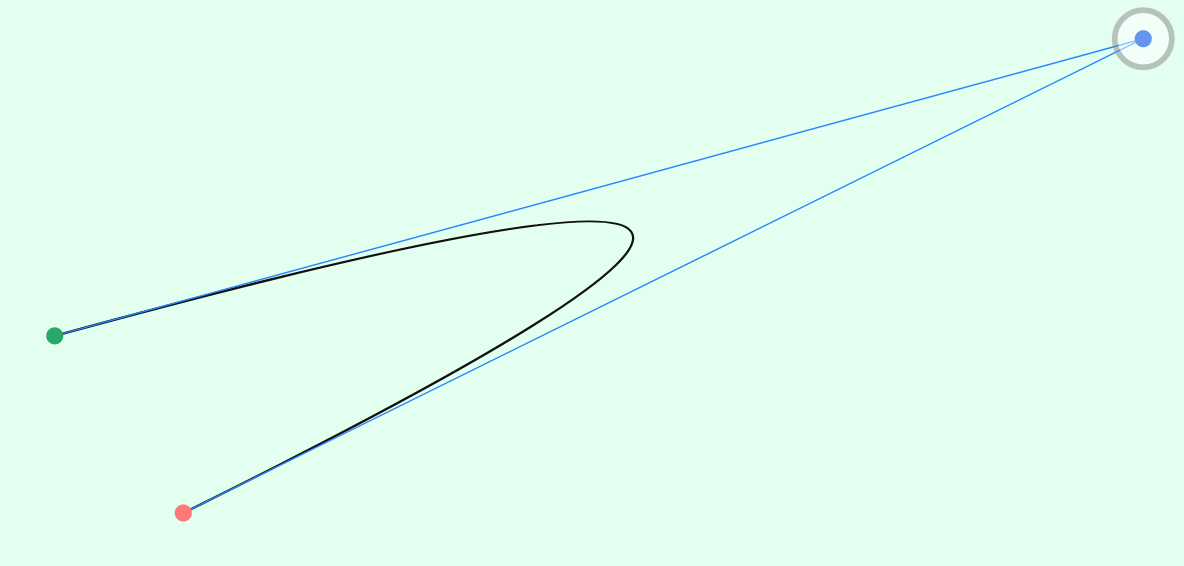
\includegraphics[width=0.75\textwidth]{high_curvature_stroke.png}
    \caption{«Мазок» с высокой степенью искривлённости}
    \label{fig:high_curvature_stroke}
\end{figure}
\FloatBarrier

\begin{figure}[h!]
    \centering
    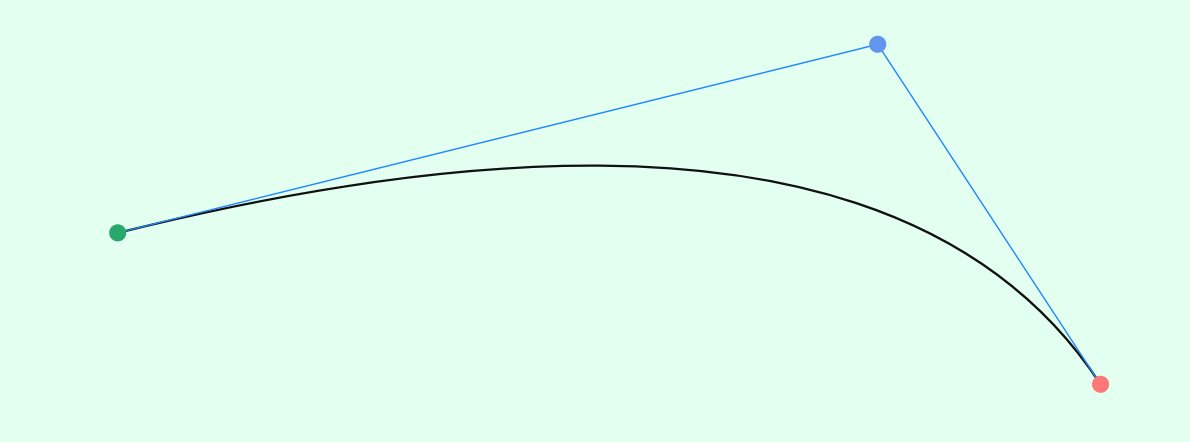
\includegraphics[width=0.75\textwidth]{low_curvature_stroke.png}
    \caption{«Мазок» с низкой степенью искривлённости}
    \label{fig:low_curvature_stroke}
\end{figure}
\FloatBarrier

Отсюда вытекает и очевидный способ уменьшить кривизну: переместить срединную точку так, чтобы она была достаточно блика к отрезку.
Нужно приблизить её в нужное количество раз по направлению либо к основанию перпендикуляра,
либо к концу отрезка в зависимости от того, куда попадает перпендикуляр.


\subsection{Сортировка мазков перед выпуском}\label{subsec:stroke_sorting}

В случае растеризации набора мазков на компьютере время выполнения операции почти совсем не зависит от порядка следования мазков
(если не считать незаметное влияние кэширования в процессоре), так как закрашивание пикселя происходит через \textit{random access}.
Однако в реальности это далеко не так: правильный порядок мазков (как по координатам, так и по цветам) может сильно уменьшить время отрисовки, которое весьма велико,
и поэтому нельзя забывать про задачу правильного расположения мазков.

\subsubsection{Сортировка по территориальному признаку}
В первом приближении количество цветов очень небольшое (скорее всего, не больше десяти),
а, чтобы сменить цвет, нужно вести кисть к банке с водой, смывать краску предыдущего цвета, брать новый,
а потом опять несть кисть через весь стол.
Поэтому разумно сначала разделить мазки на группы по цветам, а в каждой из них располагать их так,
чтобы минимизировать пройденное кистью расстояние при последовательной отрисовке мазков этого цвета.

По сути это модификация \href{https://en.wikipedia.org/wiki/Travelling_salesman_problem}{задачи Коммивояжёра}, где в роли городов выступают мазки.
Разница в том, что мазки гораздо более некорректно считать материальными точками: их размер — порядка расстояний между ними.
То есть «вход» в мазок находится с одной стороны, а «выход» — с другой, причём для каждого мазка появляется два варианта его проведения —
с одной стороны и с другой.

Конечно, можно оформить нахождение лучшей последовательности как оптимизационную задачу,
где параметрами будут:
\begin{itemize}
    \item Некая перестановка идентификаторов всех мазков
    \item Вектор бинарных величин для каждого мазка (с какой стороны начинать его рисование)
\end{itemize}

Но это будет неоправданно ресурсозатратно, так как от решения этой задачи зависит только скорость рисования, но не качество конечного продукта.

В качестве простого и быстрого алгоритма напрашивается обход «змейкой»: сортировать мазки сначала по одной координате, затем - по другой
(в качестве якорной точки разумно использовать точку $\vec{p} = bezierCurve(t = 0.5)$ (смотреть по формуле \ref{eq:bezier_curve})).
Однако на практике первая координата примерно никогда не совпадает у нескольких мазков, поэтому сортировка по сути происходит только по ней,
что приводит к постоянному метанию с одной стороны холста на другую.

Потому разумнее разделить изображение на прямоугольные зоны такого размера,
чтобы количество зон было порядка количества мазков в зоне, тогда делений по одной координате: $\approx \sqrt[4]{\lVert strokes \rVert}$.
Далее можно произвольно выбрать порядок мазков внутри каждой зоны: будет гарантироваться, что между каждыми мазками будет пройдено расстояние

\begin{equation}\label{eq:movement_restriction}
    \leq \sqrt{\left( \frac{image_{height}}{n_{separators}} \right)^2 + \left( \frac{image_{width}}{n_{separators}} \right)^2}
\end{equation}

Как вариант — запустить алгоритм оптимизации внутри каждой зоны: здесь, как проверено на похожих данных в репозитории PowerfulGA
возможно почти моментально получить хороший, скорее всего — идеальный — результат.

Сейчас используется разбиение на зоны с дальнейшей сортировкой по одной из координат.

Такой способ даёт удовлетворительное качество, однако рассматривается использование
\href{https://en.wikipedia.org/wiki/Christofides_algorithm}{алгоритма Кристофидеса} —
возможно, он даёт более хорошее качество (гарантирует длину пути не более, чем в 1.5 раз больше минимального).

\subsubsection{Оптимальная расстановка цветов}\label{subsubsec:color-sequence}

Когда внутри каждого цвета мазки расставлены, встаёт ещё один вопрос: как должны быть упорядочены сами цвета.
По разным причинам предпочтительно делать это в «хронологическом», «плавном» порядке — чтобы близкие цвета
сильно не отличались и мы постепенно переходили от одной крайности к другой.
Это и уменьшает артефакты при использовании нового цвета после старого,
и (в перспективе, когда будут масляные краски) необходимо для смешения.
Более того, это полезно для получения итоговых цветов (см.~\ref{subsec:getting-final-colors})

Здесь полезно представление цвета как вектора в трёхмерном пространстве (компоненты вектора нём — это компоненты R, G и B).

Далее необходимо формализовать задачу.
Есть несколько вариантов выбора целевого функционала:
\begin{itemize}
    \item Непосредственно, длина ломанной
    \item Сумма квадратов длин отрезков ломанной.
    Этот вариант предпочтительнее, так как дополнительно наказывает за большие промежутки между цветами
    (то есть стимулирует равномерность в последовательности).
\end{itemize}

В первом случае мы снова получаем задачу Коммивояжёра, а во втором — просто некую оптимизационную задачу.
Причём отжигом её решать уже целесообразно, так как количество цветов обычно не больше 1000.


\subsection{Получение итоговых цветов: сжатие палитры}\label{subsec:getting-final-colors}
Чтобы реальный робот быстро рисовал изображения из реальной жизни (а не тестовые),
количество используемых цветов должно быть невелико (скорее всего, не больше десяти).
Однако сейчас генерируется большое количество цветов, и у мазков редко каких зон цвета совпадают.
Нужно без потери качества «сжать» палитру — каждому изначальному цвету сопоставить один из немногих новых.

Ориентировочное количество цветов (целевой размер палитры) задаётся пользователем исходя из физических ограничений робота
(на самом деле, в результате количество цветов будет в точности равно этому числу).

Имея «плавную» последовательность цветов (из~\ref{subsubsec:color-sequence}),
можно использовать её для сжатия палитры: алгоритм очевиден.

Измерим полученную длину пути от первой до последней точки (в трёхмерном цветовом пространстве)
или сумму квадратов расстояний между последовательными точками (в зависимости от того, какая метрика выбрана).
Назовём полученное значение $L$.
Затем будем двигаться по последовательности цветов, поддерживая счётчик сумм длин или их квадратов,
и каждый раз проверять, не достигли ли мы значения $\frac{L}{n}$, где $n$ — количество цветов.
При достижении переходить к добавлению в новую группу.
Так мы разделили цвета на группы близких.
Осталось в каждой выбрать цвет, наилучшим образом представляющий изначальные цвета, собравшиеся в этой группе.
Как было показано в~\ref{subsubsec:optimal-color-finding}, для этого достаточно составить цвет из средних арифметических по каждой компоненте.

\subsection{Соотнесение параметров с физическими величинами}\label{subsec:physical-values}
Были проведены измерения толщин кисти, калибровка и т.д.
Размеры задаются через среднее геометрическое и размер диапазона (в «разах»):

\begin{equation}
    min_p = \frac{g_{avr}}{\sqrt{range\_size}}
\end{equation}

\subsection{Учёт специфики кисти}\label{subsec:brush-specific}

В ходе запусков выяснилось, что робот не может рисовать короткие, но толстые мазки.
Поэтому было решено изменить параметры, находящиеся в геноме.
Теперь будет храниться не $width$, а $fatness$ — отсылка к тому, что для человека с бо́льшим ростом выше максимальный порог приемлемой толщины тела.

Сделано это для того, чтобы ни при каких значениях генома, входящих в указанный диапазон, не было тонких и коротких мазков.

Теперь достаточно задать трёхмерную функцию, которая по $fatness$ и рассчитанной длине мазка находит $width$.
Например, при очень большой длине верхняя грань ширины для разных значений $fatness$ — это толщина кисти при максимальном нажатии.

Такой подход — принципиальная альтернатива методу с «корректировкой».
В случаях, когда можно, чтобы на всём допустимом множестве значений, указанном алгоритму оптимизации,
генерировалась потенциально приемлемая картинка.

Это будет реализовано в ближайшее время.
